\chapter{背景}

\section{大規模言語モデル（LLM）における感情表現}

\subsection{離散的感情ラベルとその限界}

初期の研究では、感情は少数の離散的カテゴリの集合として扱われていた。最も影響力のある分類体系は、Ekmanの7つの基本感情、すなわち怒り・軽蔑・嫌悪・喜び・恐怖・悲しみ・驚きである~\cite{ekman1999basic}。

\begin{figure}[H]
    \centering
    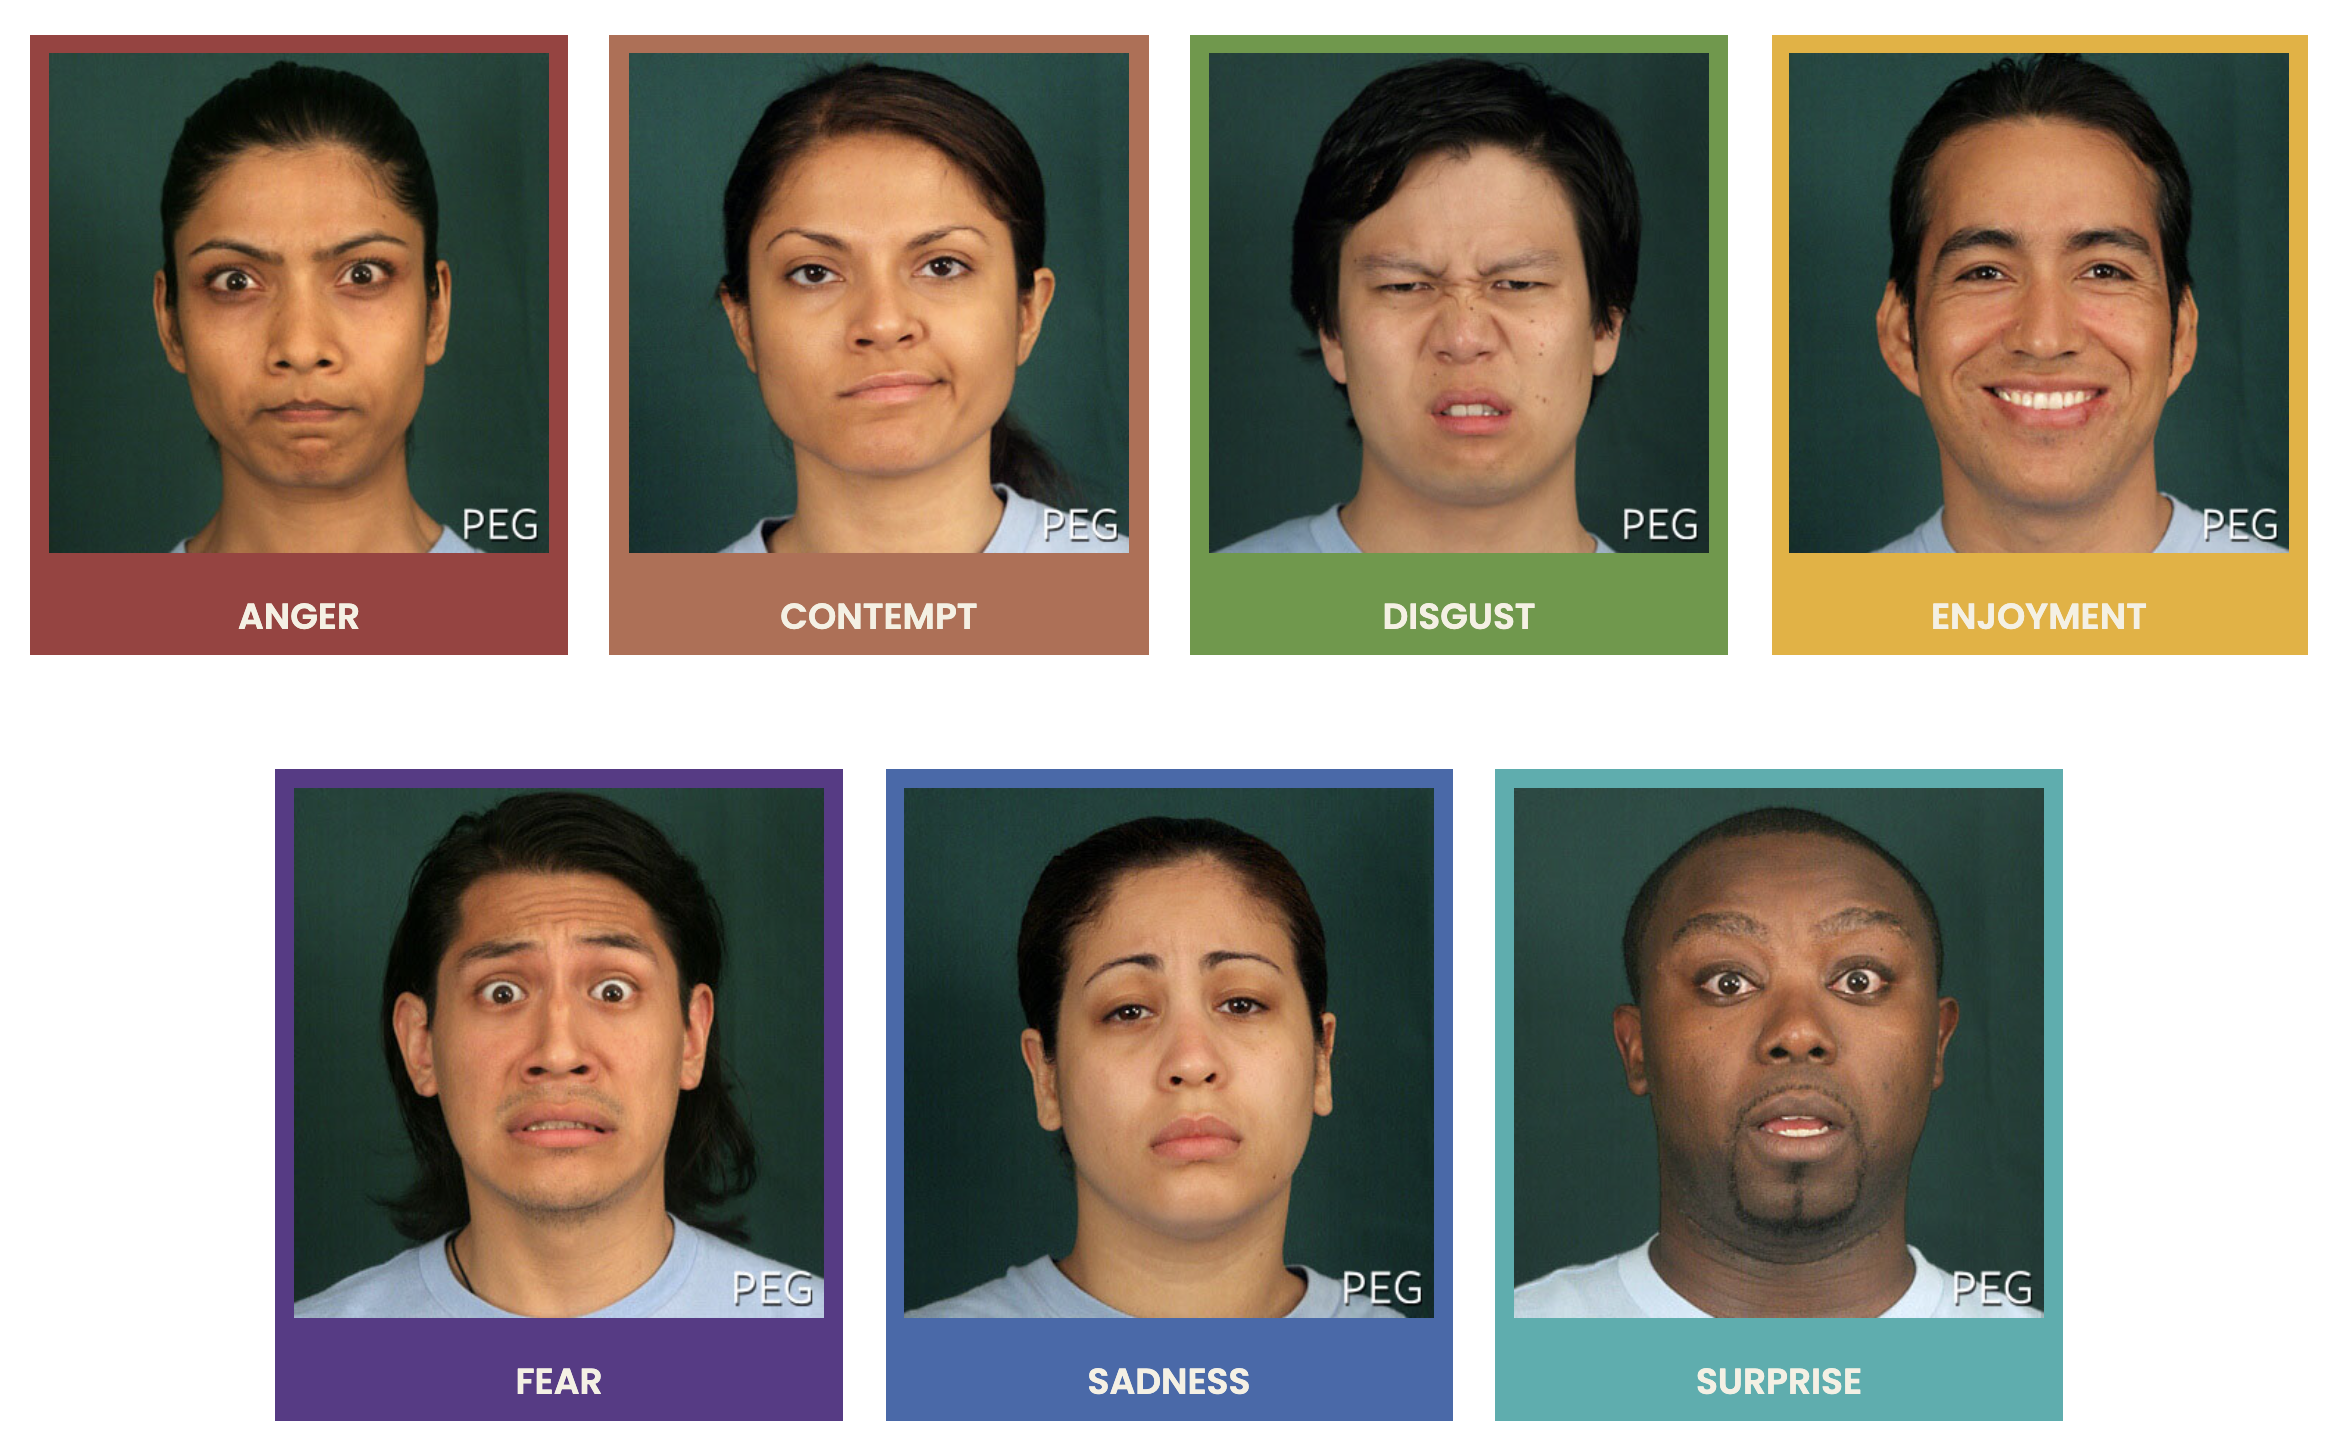
\includegraphics[width=0.5\linewidth]{figures/paul_ekman.png}
    \caption{Paul Ekmanの7つの基本感情~\cite{paul_ekman_web}}
    \label{fig:paul_ekman}
\end{figure}

この枠組みは、感情が生物学的に普遍的かつ心理学的に還元不可能であると仮定するものである。明確なラベリング体系を提供することで、初期の教師あり感情分類システムを可能にし、ベンチマークデータセットの構築を促進した。しかしながら、カテゴリ的仮定は強い帰納的バイアスをもたらす。すなわち、感情は互いに排他的かつ質的に独立したものとして扱われる。

その後のデータセットは表現の粒度を高めようと試み、様々なドメインにわたる情動的理解を測定するベンチマークタスクが確立された~\cite{mohammad2018semeval}。たとえば、GoEmotions~\cite{goemo}はラベル空間を27の感情カテゴリに拡張し、マルチラベルアノテーションを可能にした。

\begin{figure}[H]
    \centering
    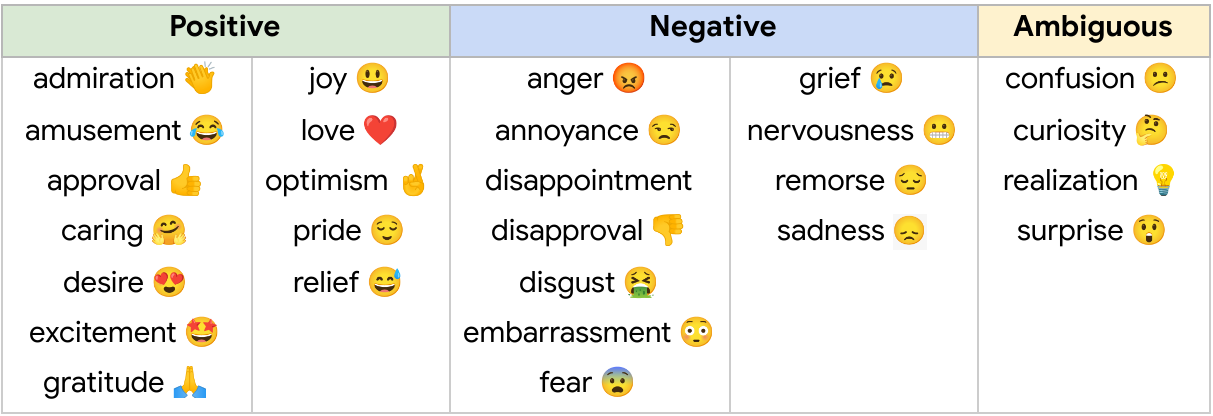
\includegraphics[width=0.8\linewidth]{figures/goemotions.png}
    \caption{GoEmotionsの分類体系：``neutral''（中立）を含む28の感情カテゴリ~\cite{goemo}}
    \label{fig:goemotions}
\end{figure}

これにより、1つの発話に複数の感情が生じる事例を捉えることが可能になった。感情は感情極性と強度によってクラスタリングされ、多くのカテゴリが高いラベル間相関を示すことが報告されている。しかしながら、表現解像度が向上したにもかかわらず、このデータセットは依然としてワンホット／スパースなマルチホット符号化に依存している。このような符号化は、感情の強度と合成的構造を離散的なインデックスに圧縮してしまい、段階的な遷移の表現を妨げる。たとえば、穏やかな怒りと強烈な怒りの違いは表現できず、苦くも甘い（bittersweet）感情のような感情の混合も困難である。

本質的に、離散ラベルは学習問題を連続性・幾何学的構造・算術的構造を捉えることのできない分類の枠組みに押し込めてしまう。たとえば、\texttt{joy}（喜び）とラベルされた2つのサンプルが感情的に遠い場合もあれば、\texttt{joy}と\texttt{contentment}（満足）が感情的に近い場合もあるが、このような構造はモデル自体には不可視のままである。これらの限界は、純粋にカテゴリ的な表現から連続的感情空間への移行を動機づける。

離散化された感情ラベルのこの問題は、Wang and Zong (2021)~\cite{wang-zong-2021-distributed}によっても提起されている。彼らはワンホット感情ラベルが感情カテゴリ間の潜在的な関係を無視していると主張することで、これを明示的に定式化している。感情クラスは人間の知覚において直交していないのではなく、段階的な様式で類似性を示すと彼らは観察している。より広い観点では、離散ラベリング体系はアノテーションの利便性を表現の妥当性より優先しており、感情の根底にある構造を曖昧にする人工的な境界を課している。このミスマッチは、ラベル粒度の違いが純粋なカテゴリ的枠組みの中で調整できないデータセット横断的転移や異文化間比較を試みる際に特に問題となる。

これらの限界は、本研究における具体的な決定を形づくる。すなわち、感情を分類ターゲットとして扱うのではなく、ここでの実験は感情を活性化空間における連続的な方向としてプロービングし操作する。次のサブセクションでは、このアプローチが基盤とする連続表現を概観する。

\subsection{離散ラベルから連続的感情空間へ}

連続的感情表現は、感情を低次元ベクトル空間における点として符号化することを目指す。この空間では、距離・方向・大きさが心理学的な関係性に対応する。感情価（バレンス）--覚醒度（アラウザル）--支配性（VAD）枠組み~\cite{MehrabianRussell1974}のような初期の心理学的モデルは、感情をカテゴリ的にではなく量的に異なるものとして示唆しながら、感情を連続軸に沿って定式化した。これらの次元に関する経験的基準値は、その後大規模な語彙集~\cite{mohammad2025nrcvadlexiconv2}にまとめられている。

\begin{enumerate}
    \item \textbf{感情価（Valence／Pleasure）}は、不快から快適にわたる経験の快楽的質を表す。喜び・満足・充実感などの状態は感情価軸の正の端に位置し、悲しみ・嫌悪・絶望は負の端に向かって位置する。
    \item \textbf{覚醒度（Arousal）}は、穏やかあるいは無気力から興奮あるいは動揺にわたる、感情状態に関連した生理的・認知的活性化の程度を捉える。高覚醒状態には恐怖・怒り・興奮が含まれ、低覚醒状態にはリラクゼーション・倦怠感・憂鬱が含まれる。
    \item \textbf{支配性（Dominance）}は、個人が状況を制御していると感じる程度、あるいは状況に圧倒されていると感じる程度を反映する。高支配性の状態は主体感・自信・制御感（例：誇り・怒り）と関連し、低支配性の状態は服従・無力感・脆弱性（例：恐怖・恥）に対応する。
\end{enumerate}

これら3つの次元を合わせると、標準的な感情カテゴリが点ではなく領域に対応する連続的情動空間が定義される。たとえば、怒りと恐怖はいずれも負の感情価を持ち高覚醒だが、支配性の軸に沿って分離可能である。悲しみと倦怠感は低覚醒と負の感情価を共有するが、支配性と強度において異なる。この幾何学的解釈は、段階的な感情強度・混合感情・情動状態間の滑らかな遷移を自然に説明する——離散ラベルでは表現が困難な現象である。

\begin{figure}[H]
    \centering
    \includegraphics[width=0.8\linewidth]{figures/PAD.png}
    \caption{立方体を用いたVADモデルの表現~\cite{PAD}}
    \label{fig:VAD}
\end{figure}

さらに、情動的計算の分野では、離散ラベルと連続的感情表現の間のギャップを橋渡しする明示的な試みがBuechel et al.~\cite{buechel2021labelagnosticemotionembeddings}によって提示されている。単一の感情分類体系に縛られるのではなく、彼らは極性・基本感情カテゴリ・感情価や覚醒度などの情動的次元を含む異種アノテーション体系にわたる共有潜在表現として機能する\textbf{ラベル非依存感情埋め込み}の学習を提案している。

重要なことに、この枠組みにおける感情ラベルは直接予測すべきターゲットとして扱われるのではなく、共通埋め込み空間からの射影として扱われる。モデルはテキストをこの潜在的情動空間にマッピングするよう訓練され、そこから軽量な予測ヘッドを介して複数のラベル形式を復元できる。この設計により、学習された感情情報をモデル全体を再訓練することなく別の形式に転移させることが可能になる。経験的に、Buechel et al.\ はこのような埋め込みが予測品質を保ちつつデータセット横断的な汎化を支援することを示している。

これを補完する形で、Wang and Zong (2021)~\cite{wang-zong-2021-distributed}は感情カテゴリ自体の連続表現を学習することに焦点を当てている。感情クラスをワンホットベクトルで表現する代わりに、彼らは特定の感情カテゴリのすべてのインスタンスにわたってソフト分類器の出力を平均化することで分散感情埋め込みを導出する。これらの表現は、テキストで表現される感情間の経験的類似性が距離に反映される感情空間を形成する。彼らの結果は、感情カテゴリが感情極性と強度によってクラスタリングされることを示しており、これは従来の意味的単語埋め込み空間よりも忠実に感情を捉えている。

重要なことに、感情を連続空間で表現することは、学習問題を硬直した分類から幾何学的表現学習へと移行させる。これは離散ラベルに内在する多くの限界を解決するだけでなく、ベクトル表現において感情情報がどのように符号化されるかをより一般的に分析するための基盤も提供する。特に、感情が学習された埋め込み内で識別可能な部分空間や線形方向を占めるかという問いを提起する。この問いは次のサブセクションで探求される。

\subsection{単語埋め込み空間における感情の線形構造} \label{linear_word_embedding_ja}

大規模言語モデル（LLM）が登場する以前から、静的な単語埋め込みは明示的な感情的監督なしに訓練されているにもかかわらず、潜在的な情動的組織化の証拠を示していた~\cite{radford2017learninggeneratereviewsdiscovering}。

Wu and Jiang~\cite{linear_vector_emo}は、GloVe~\cite{pennington2014glove}などの単語埋め込みにおける感情情報が次元全体に均一に分布しているのではなく、少数の線形方向に沿って集中していることを示す。彼らはアノテーション付きナラティブデータ上で連続的な感情価を予測する線形自己回帰モデルを訓練し、埋め込み次元の限られた部分集合のみが感情価に寄与することを示している。学習された重みを解釈すると、感情極性が完全な意味空間内に埋め込まれた低次元部分空間によって捉えられることが明らかになる。

また、単語埋め込みをこの学習された感情部分空間に射影すると、正と負の感情の間の分離が著しく明確になることも報告されている。これは、埋め込みが情動的目標なしに訓練された場合でも、感情が線形に復元可能であることを示している。すなわち、感情的意味は語彙的連想の副産物ではなく、幾何学的に符号化されているということだ。

特に重要な発見は、\textbf{この射影された感情空間が線形合成的構造を保持している}という点である。感情を含む単語に対するベクトル演算は合成的情動状態を生み出す。これはPlutchikの感情の輪~\cite{plutchik1980emotion}のような感情合成の心理学的理論とも一致している。

\begin{figure}[H]
    \centering
    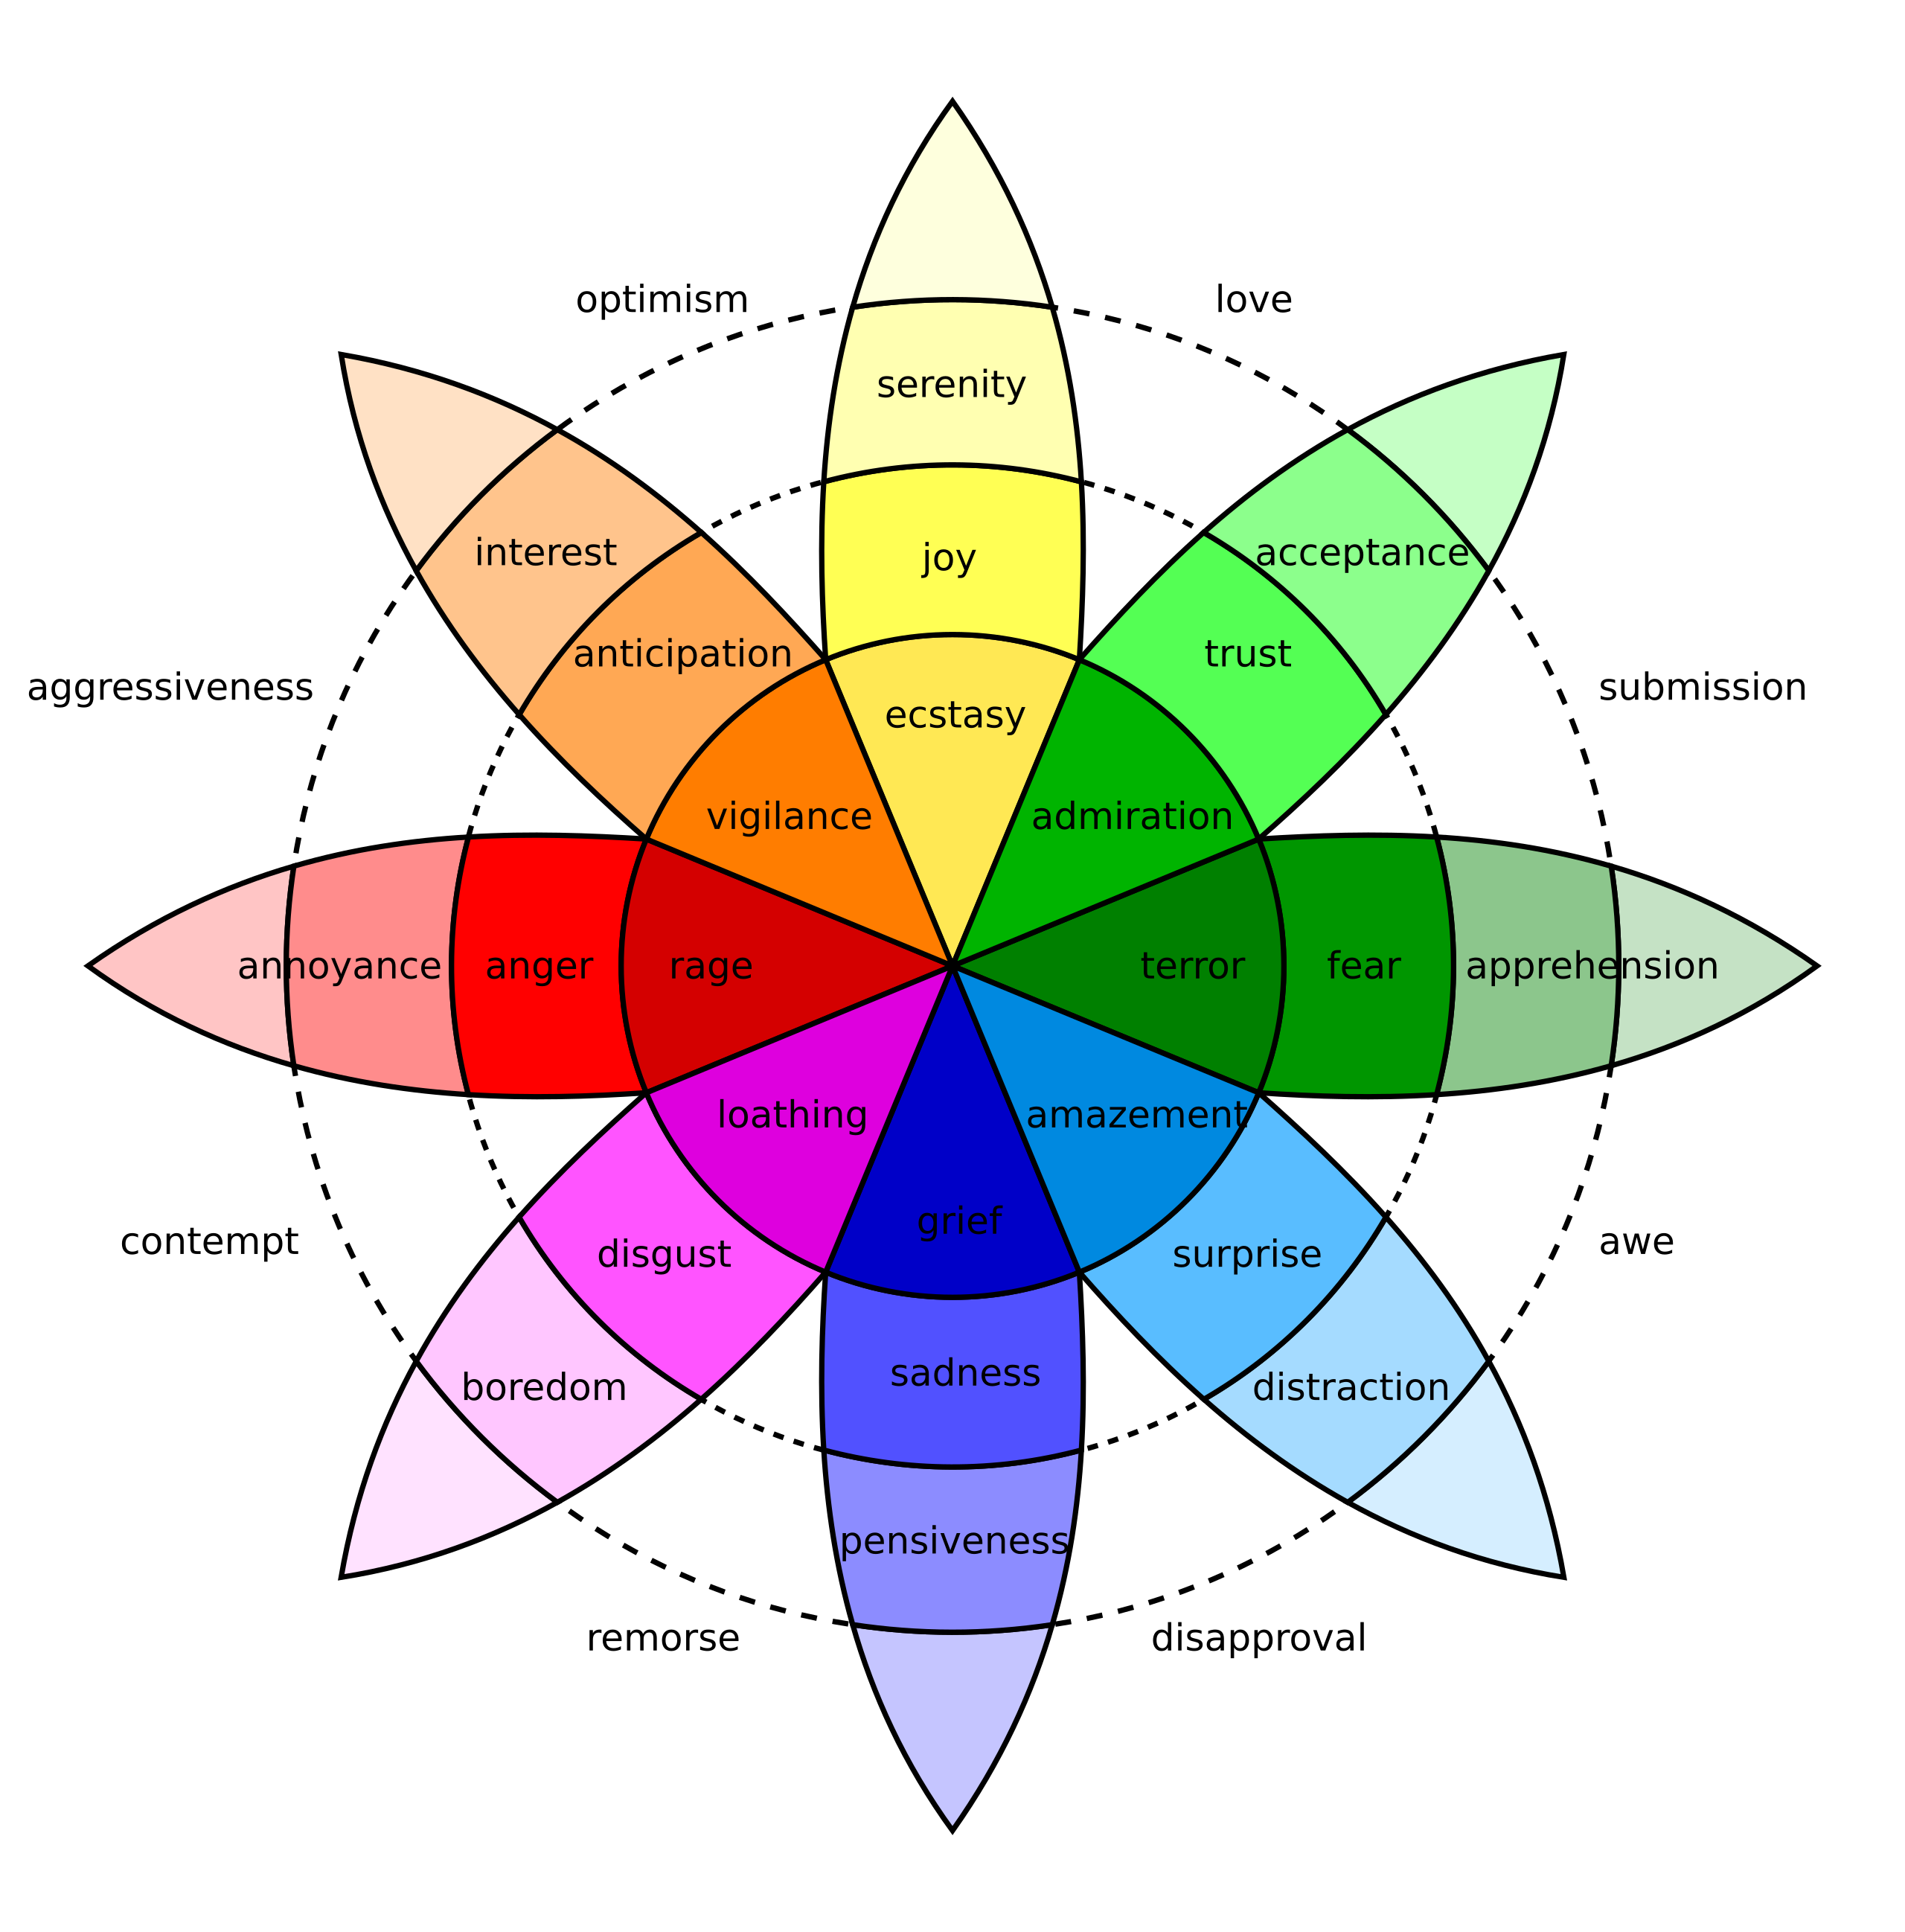
\includegraphics[width=0.5\linewidth]{figures/Plutchik-wheel.png}
    \caption{Plutchikの感情の輪：基本感情は放射状に配置され、角度的近さが類似性を、半径方向の強度が感情的強さを示す。}
    \label{fig:Plutchik}
\end{figure}

たとえば、\texttt{joy}（喜び）と\texttt{trust}（信頼）のベクトル和は\texttt{love}（愛）と密接に一致し、\texttt{remorse}（後悔）のような情動的に対立する状態からは遠い位置に留まる。この挙動はカテゴリ的表現では捉えられないが、連続的なベクトル値枠組みでは自然に現れる。

これらの結果は、単語埋め込み空間における感情が連続的であるだけでなく近似的に線形でもあり、意味のある射影・方向・算術演算を許容することを示している。その結果、情動的類似性・強度・合成は、離散的クラス境界ではなく単純な線形演算を通じて表現できる。

まとめると、これらの発見は感情が学習された言語表現内で構造化された幾何学として符号化されているという初期の証拠を提供する。これは感情の心理学的モデルと数学的埋め込みパラダイムの間に表現論的な橋を架ける。また、このような線形感情構造がより表現力豊かな表現学習システムでどのようにスケールし発展するかについてのさらなる研究を動機づける。

\section{トークンベース推論の限界}

従来の大規模言語モデル（LLM）はトークン空間で推論する。入力は人類が「語彙」として引いた離散的境界に射影されるため、細やかな情動的ニュアンスや身体化された微妙さはその射影において取り返しのつかない形で失われ、ある出力言語に残るものと別の言語に残るものは異なる場合がある。語調を調整するためにプロンプトエンジニアリングや命令チューニング（「丁寧に答えてください」など）がよく使用されるが、遵守は不確実で細粒度の制御は困難だ。他の対策としては、スタイルを内在化するための教師ありファインチューニングや、ラベル条件付き生成（例：\texttt{<joy>}や\texttt{<sad>}を追加する）が含まれるが、ファインチューニングはコストがかかりスタイル間の切り替えは柔軟性に欠ける。ラベル条件付けもまた、複雑なニュアンスの混合を捉えることができない。

情動的制御を超えて、推論自体にも同じ限界が適用される。自己回帰型言語モデルは、生成プロセスにおいてトークンの機能を考慮しない。たとえトークンが重要な推論内容を担っていても、\texttt{a}や\texttt{is}のような文法的トークンとほぼ同じ計算予算が割り当てられる。その結果、内部状態のごく一部だけが実際の推論作業を担い、明示的な推論トレースのほとんどのトークンは根底にある計算に寄与しない。

最近の研究はこの表層的な出力トークンと内部推論プロセスの間の断絶を示している。Pfau et al.\ (2024)~\cite{pfau2024lets}は、出力トークンが意味的に無情報であっても、トランスフォーマーが非自明な隠れた計算を実行できることを示している。たとえば、フィラーや一時停止トークン（明示的な意味を持たない）を挿入することで、推論タスクのパフォーマンスが測定可能な形で向上する。これは、本質的な計算が発行されるトークン自体ではなく潜在的な活性化によって担われていることを示唆している。トークン生成は、内部プロセスの周囲にある通信的言語制約に過ぎない。

トークンベース推論の非効率性は、推論が明示的に言語化される際に一層明らかになる。思考の連鎖プロンプティングは多くのタスクでパフォーマンスを向上させるが、\textbf{それらの状態が本来言語的でない場合でも、モデルに中間状態を自然言語に外部化させることを要求する}。Hao et al.\ (2025)~\cite{hao2025traininglargelanguagemodels}が主張し、推論を連続空間に圧縮することに関する関連研究~\cite{shen2025codicompressingchainofthoughtcontinuous}によって裏付けられているように、言語は計算ではなくコミュニケーションのために最適化されている。推論を離散語彙の制約内で展開させることは、不必要なオーバーヘッドと歪みをもたらす。多くの推論トークンは推論に必要だからではなく、人間の可読性のために必要なのだ。

この観点から、明示的な言語化は前のセクションで議論した情動的推論に対する非可逆圧縮の一形態を構成する。推論中の連続的かつ高次元の内部状態は、離散的かつ文化的に依存したトークン空間に射影されなければならず、これは計算にとっては可視でも単語レベルでは不可視の区別を平坦化する。感情構造は本質的に段階的であり、正確な語彙化に抵抗するため、この圧縮は情動的計算にとって問題となる。

まとめると、これらの観察はトークン空間が推論の基盤ではなく、むしろインターフェースであることを示唆している。コミュニケーションと監督のための便利な媒体を提供する一方で、内部計算には最適ではない。これは、大規模言語モデル（LLM）の感情的行動を理解し制御するために潜在表現を直接調べることを動機づける。これが次のセクションの焦点である。

\section{潜在表現の操作}

感情が潜在空間において幾何学的に符号化されていること、そしてトークンベースのインターフェースがこの連続的構造を忠実に表現できないことの両方を確立した上で、ここではモデルのこれらの内部表現を直接操作する技術に目を向けたい。

\subsection{大規模言語モデル（LLM）における創発的感情部分空間}

大規模言語モデル（LLM）は、静的な単語埋め込みで以前に観察された情動的構造（\ref{linear_word_embedding_ja}）を大幅に拡張・一般化する。モデルが感情情報の監督なしに大規模コーパスで訓練されているにもかかわらず、大規模言語モデル（LLM）は豊かな文脈的表現を獲得している。これらのモデルは感情を隠れ状態の幾何学の連続的かつ分散的な特性として内在化しているように見える。

最近の研究はこの主張に対する強い経験的証拠を提供している。Reichman et al.\ (2025)~\cite{reichman2025emotionsartthouunderstanding}は、大型のデコーダのみの大規模言語モデル（LLM）における感情情報が活性化に埋め込まれた低次元の\textbf{感情多様体}内に組織化されていることを示している。

彼らは層をまたいで隠れ状態を分析し、情動的内容が少数の安定した潜在方向にどのように整合するかを示した。重要なことに、これらの方向は明示的な感情的監督なしに現れており、情動的構造がタスク固有のアーティファクトではなく大規模言語モデリングの自然な結果であることを示している。さらに、識別された感情部分空間はドメインと言語にわたって著しく一貫しており、大規模言語モデル（LLM）が広く普遍的な情動的幾何学を内在化していることを示唆している。

重要なことに、この幾何学は単に記述的なものではない。Reichman et al.~\cite{reichman2025emotionsartthouunderstanding}は、これらの潜在方向に沿った小さな介入がモデルの入力に対する感情的解釈を変えながら意味的内容を保持できることを示している。これにより、感情部分空間は表層レベルの感情的手がかりの受動的相関関係ではなく、モデルの表現空間の機能的に意味のある構成要素として確立される。

補完的な証拠はニューロンレベルの分析からも得られる。Lee et al.\ (2025)~\cite{lee-etal-2025-large}は、大型の命令チューニング済みモデルにおいて特定の基本感情を選択的に追跡する活性化を持つニューロンのグループを同定している。感情情報は広く分布しているが、特定のニューロンは特定の情動状態に対して常に不均衡に強い反応を示す。さらなるアブレーション実験により、これらのニューロンを抑制すると一部の感情に対する感情認識パフォーマンスが著しく低下することが明らかになった。これは感情情報が副現象的ではなく能動的に処理されているという因果的証拠を提供する。

まとめると、これらの発見は大規模言語モデル（LLM）における感情が高次元の文脈的表現に埋め込まれた創発的な低次元部分空間として最もよく特徴づけられることを示唆している。感情的意味は単一のユニットに局在するのでも離散ラベルに還元可能なのでもなく、安定した潜在空間の構造化された領域を占めている。この創発的情動幾何学は、線形介入を通じた感情的行動の直接制御を可能にする表現論的基盤を提供する。これについては次で議論する。

\subsection{コントラスティブ活性化加算による潜在状態のステアリング}

大規模言語モデル（LLM）における感情的意味が潜在表現内の方向や部分空間として符号化されているならば、自然な帰結として、情動的行動はそれらの方向に沿って介入することで直接制御可能であるべきである。この観察は、推論中に内部活性化に線形かつ連続的な制御ベクトルを直接適用する\textbf{潜在ステアリング}に関する一連の研究を動機づけている。

初期の影響力のあるアプローチはプラグアンドプレイ言語モデル（PPLM）~\cite{dathathri2020plugplaylanguagemodels}であり、これは凍結された大規模言語モデル（LLM）と外部属性モデル（例：感情分類器）を組み合わせ、望ましい属性の尤度を高めるために隠れ状態に対して勾配上昇を実行する。実質的に、この方法は\textbf{感情ベクトル}を潜在表現に導入し、モデルの重みを修正することなく生成を正または負の感情に向けてバイアスする。もともと制御可能な生成技術として組み立てられていたが、PPLMは情動的属性が潜在空間の近似的に線形な方向に対応するという仮定に暗黙的に依存している。

より最近の研究はこの仮定を明示的にし、反復的最適化の必要性を除去している。AnthropicのCAA（コントラスティブ活性化加算）~\cite{caa}は、事前計算された\textbf{ステアリングベクトル}を使用してモデルの内部活性化に直接介入する。ステアリングベクトルの構築手順は2つのフェーズからなる。まず、コントラスティブデータセットが構築される。すなわち、ターゲット行動を引き出す\textit{正例}プロンプトの集合と、そうでない対応する\textit{負例}プロンプトの集合である。情動的ステアリングの場合、これは喜びに満ちたバージョンと悲しいバージョンのような、感情的な語調のみが異なる文ペアを通じて実現される。次に、モデルは各プロンプトペアを処理し、指定された層$l$における隠れ状態の活性化の差が計算される。これらの差はデータセット全体で平均化され、単一のステアリングベクトル$\mathbf{v}_l$が生成される：

\begin{equation}
    \mathbf{v}_l = \frac{1}{N}\sum_{i=1}^{N}\left(\mathbf{h}_l^{(+,i)} - \mathbf{h}_l^{(-,i)}\right)
\end{equation}

\noindent ここで$\mathbf{h}_l^{(+,i)}$と$\mathbf{h}_l^{(-,i)}$はそれぞれ$i$番目の正例と負例プロンプトについての層$l$における隠れ状態を表す。推論中、ステアリングベクトルは各順伝播において残差ストリームに加算的に注入される：

\begin{equation}
    \mathbf{h}_l \leftarrow \mathbf{h}_l + \alpha\,\mathbf{v}_l
\end{equation}

\noindent ここで$\alpha$は介入の強さと方向を制御するスカラー乗数だ。$\alpha$の正の値はターゲット属性に向けてステアリングし、負の値はそれから離れる方向にステアリングする。

CAA（コントラスティブ活性化加算）の主要な利点はその単純さと解釈可能性にある。介入は線形であり、効果の強さは$\alpha$をスケーリングすることで連続的に変調できる。さらに、複数のステアリングベクトルを加算的に組み合わせることができ、複数の属性に対する合成的制御が同時に可能になる。プロンプトエンジニアリングやファインチューニングとは対照的に、このような介入はモデルの内部状態に直接作用し、特に感情や感情的語調のような抽象的特性に対してより正確かつ堅牢な制御をもたらすことが多い。

元のCAA（コントラスティブ活性化加算）論文の実験は、このアプローチが感情・追従性・拒否行動を含む様々な属性にわたってターゲット行動を確実に誘発することを示している。重要なことに、ステアリングの効果は層全体で均一ではない。最初や最後の層ではなく、トランスフォーマーの中間層に介入が適用される場合に、より強力で一貫した効果が観察される。この層感度は大規模言語モデル（LLM）における情動的情報の階層的組織化に関する発見と一致している。下位層は表層的な語彙的特徴を符号化し、中間層は感情的意味を包含する文脈的・意味的構造を統合する。

重要なことに、潜在状態のステアリングは表層レベルの語彙的選択にのみ影響するのではない。中間層に情動的制御ベクトルを注入することで、モデルの感情的文脈の内部解釈を変え、感情的手がかりがネットワークの後続層を通じてどのように統合され伝播されるかを変更できる。これは大規模言語モデル（LLM）における感情が個々のトークンや出力に結びついた特性ではなく、グローバルな潜在変数として機能するという見方を支持する。

この層感度は、前のセクションで議論したトークンベース表現の限界と並べて見ると、より深い含意を持つ。ステアリングが最も効果的であることが証明される中間層は、まさに情動的情報が抽象的・意味的構造として組織化される層である——内部状態を特定の語彙選択にマッピングする下流プロセスに先立つ順伝播の段階である。このレベルでのステアリングは、したがって\textbf{前言語的感情状態}への介入を構成する。すなわち、モデルの感情の表現がいかなる単語やフレーズも完全に表現できるよりも豊かで連続的な段階である。

この区別は重要である。プロンプトエンジニアリングや命令チューニングのようなトークンレベルの介入は必然的に離散語彙の制約内で動作し、語彙選択のボトルネックを通じて感情的ニュアンスを強制する。これに対して、中間層に適用された情動ステアリングベクトルはそのボトルネックに達する前に内部感情状態を形成する。その結果の出力は、直接的な表現に抵抗しながらも読者には知覚可能な微妙な感情の段階性を反映できる——真に名付けることが困難だが、語調・語順・リズムの中で紛れもなく存在するようなニュアンスである。この意味で、層ターゲットCAA（コントラスティブ活性化加算）は前言語的感情を表現する道を提供する。すなわち、潜在空間における構造化された方向として存在するが、次トークン生成によって課される圧縮において部分的に失われることになるような情動的内容である。

さらに、CAA（コントラスティブ活性化加算）は二値的な正/負の制御を超えて情動的強度の細粒度変調を可能にする。スカラー係数$\alpha$を変化させることで、モデルを感情的連続体に沿った異なる点に向けてステアリングし、穏やかから激しい感情的表現にわたる出力を生成できる。これは感情の強度がラベル自体によって固定される離散ラベル条件付き生成とは質的に異なる。

結論として、CAA（コントラスティブ活性化加算）は大規模言語モデル（LLM）における感情制御のための原理的かつ経験的に検証されたメカニズムを提供する。その線形性・スケーラビリティ・合成可能性は、潜在空間における情動的表現の構造を調査するのに適しており、本論文で報告される実験で使用される主要な介入方法である。

\subsection{線形感情方向に関する因果的証拠}

表現空間における情動的方向の存在は線形プローブや次元削減によって示すことができるが、それらが実際にモデル行動において因果的役割を果たすかどうかはいまだ疑問が残る。最近の研究は、大規模言語モデル（LLM）における感情方向が線形的に復元可能であるだけでなく、情動的推論において機能的に必要かつ十分であるという強い証拠を提供している。

Tigges et al.\ (2024)~\cite{hollinsworth-etal-2024-language}は、大規模言語モデル（LLM）における感情が文脈的埋め込みの単一の支配的な線形方向に沿って符号化されていることを示している。彼らは方向的アブレーションと介入を実施し、この感情方向を除去/抑制することが感情分類のような下流の感情感受性タスクにおける系統的な性能低下をもたらすことを示した。逆に、同じ方向を中立的な文脈に注入することは、モデル出力の予測可能なシフトを引き起こす。この双方向的操作は、感情方向が受動的相関関係ではなくモデルによって能動的に使用されているという証拠を提供する。

重要なことに、大規模言語モデル（LLM）における情動的能力は感情関連タスクに対する明示的なファインチューニングに依存しない。Broekens et al.\ (2023)~\cite{broekens2023finegrainedaffectiveprocessingcapabilities}は、ChatGPTのような既製の大規模言語モデル（LLM）がプロンプティングのみを使用してテキストを正確な感情価（バレンス）--覚醒度（アラウザル）--支配性（VAD）値にマッピングし、細粒度の感情的手がかりを検出できることを示している。これは連続的な情動的表現が一般的な言語理解の一部として潜在空間にすでに埋め込まれていることを示唆している。これは感情をタスク固有の出力形式ではなく、前言語的潜在変数として解釈する強い証拠である。

より大きなスケールでは、感情表現が平坦ではなく階層的に構造化されていることをさらに示す証拠がある。Zhao et al.\ (2025)~\cite{zhao2025emergencehierarchicalemotionorganization}は、非常に大型のモデル（4050億パラメータ以上）が基本的な情動状態がより具体的な感情に分岐する木状の感情表現を発達させることを観察している。より一貫した階層的情動幾何学を持つモデルは感情認識能力の向上と交渉シナリオにおける説得効果の増大を示す。これは感情表現の内部構造を機能的行動に直接結びつける。

これらの発見は大規模言語モデル（LLM）における情動的幾何学の因果的解釈に収束する。感情方向を除去すると情動的推論が損なわれ、注入すると行動が予測可能に変化する。さらに、感情情報は孤立したトークンやニューロンに限定されておらず、モデルの一般的な情動的能力を形成するグローバルな潜在変数へと層をまたいで蓄積・要約される。

結論として、ベクトルベースの感情操作のための原理的な基盤があり、これによってトークンレベルの置換ではなく埋め込みに対する数値演算を通じて感情的ニュアンスを表現することが可能になる。この因果的根拠は、大規模言語モデル（LLM）における感情的行動を制御し整合させようとする本プロジェクトにとって不可欠である。

\subsection{情動的表現への含意}

上述の発展は、一貫した全体像に収束する。感情は離散ラベルや語彙的選択としてではなく、潜在表現の連続的かつ幾何学的に構造化された特性として現れる。CAA（コントラスティブ活性化加算）を通じた介入は、これらの方向が単に記述的ではなく因果的に実行可能であることを示している。すなわち、ステアリングベクトルを注入することでモデルの情動的解釈が予測可能にシフトし、意味的能力は保持される。まとめると、これは感情が表現空間において直接読み出し・操作・合成可能な内部潜在変数として機能するという見方を根拠づける。

これらの発見は、感情が表層的な出力の特性として扱われる必要はないことを示唆している。むしろ、情動的意味は順伝播全体にわたって進化する共有潜在表現に根拠を持つ。この観点から、感情情報は出力段階で適用される文体的属性ではなく、中間表現がどのように形成され伝播されるかを形成する内部推論状態自体の不可欠な部分を構成しうるものだ。

重要なことに、この可能性は大部分が未探求のままである。潜在的情動幾何学は特徴づけられ、その因果的役割は確立されているが、感情と多段階潜在計算の間の相互作用は系統的に調査されていない。感情次元が潜在推論の軌跡と整合するか、あるいは相互作用するかどうかは未解決の問いなのだ。これに対処するには、トークンレベルの分析を超えて、感情を潜在計算の第一級の構成要素として扱うことが必要だ。

これらの考察は、以降の章での調査を動機づける。感情を外部ラベルや出力制約として扱うのではなく、情動状態が推論自体の基盤となる連続的潜在空間内で表現できるという仮説を探求し——言語がもはや推論の主要な媒体でなくなった際に感情的意味がどのように持続し再表現されうるかを検討する。

%%%%%%%%%%%%%%%%%%%%%%%%%%%%%%%%%%%%
